\chapter{The Epoch of Reionization}
\label{chapter:eor_intro}

Shortly after the Big Bang, the Universe existed as an opaque, primordial soup of quarks, leptons, gluons and extremely energetic photons.
With density anisotropies formed by hugely inflated quantum fluctuations, ionized hydrogen, deuterium, helium, lithium and beryllium (but mostly hydrogen and helium) filled the Universe as a hot plasma. 
Black-body photons were continuously scattered throughout this plasma. All the while, the Universe adiabatically expanded, and the plasma cooled. 

About 380,000 years after the Big Bang, the number of photons with energies above the 13.6\,eV threshold required to ionize neutral hydrogen (astronomers refer to neutral hydrogen as {\sc hi}, and ionized hydrogen [i.e. protons] as {\sc hii}) became outnumbered by the number of baryons, and {\sc hii} was able to recapture electrons without immediately being ionized. 
During this critical period, known as recombination, the plasma was able to neutralize. The Universe underwent a cosmic transition from optically thick to optically thin as free electrons were captured, allowing light to travel unimpeded, in straight lines for the first time.
Fast-forwarding about 14 billion years (bear with me), some of these photons that existed at the time of `last scattering', redshifted by the expansion of the Universe, are observed today as the Cosmic Microwave Background (CMB).

We exist today in a structured, complicated and diverse Universe of stars and galaxies, dark matter and dark energy, but very little neutral gas. At the same time, observations of the CMB \citep[e.g.][]{Planck.16.1, Planck.16} and standard cosmological models (referred to under the umbrella term of $\Lambda$CDM, standing for Dark Energy \& Cold Dark Matter; e.g. \citet{Komatsu.09}) find extraordinary agreement with the story told above. However, there also exists a large observational gap: how did the Universe transition from it's neutral state at recombination, to its ionized and structured state today? How, and when, did the Universe \textit{reionize}?

The prevailing theory of the formation of cosmological structure begins with the primordial density anisotropies of the hot plasma. The dark matter that pervaded the Universe should have traced those perturbations, and gravitationally accreted into those regions, increasing the overdensities. Eventually, overdensities above some threshold density\footnote{For simple collapse models, this threshold is 18$\pi^2$ above the average density of the Universe; e.g. \citet{Press.74}.} collapsed into halos; structures supported by their own gravitational potential. The similarly pervasive {\sc hi} field should have traced the dark matter overdensities. This gravity-dominated period represents an epoch of relatively simple physics directly driven by $\Lambda$CDM. It is known colloquially as the ``Dark Ages", as at that time no luminous structures existed, and the only photons that existed were from the slowly fading CMB\footnote{For most purposes in this thesis, we neglect exotic physics such as Dark Matter annihilations that could in principle be an additional source of radiation at early times.}.

Within the early dark matter halos, enough {\sc hi} accreted to a great enough density to fuse, igniting the first stellar cores. These first stars (referred to by astronomers as Population-3 or ``Pop{\sc iii}" stars) were the first source of ultraviolet (UV) and X-ray photons capable of ionizing {\sc hi} since recombination. They were also extremely massive and short-lived, and their supernovae likely provided the seeds for the first galaxies (composed of Pop{\sc ii} stars; e.g. \citet{Ricotti.16}). The Pop{\sc iii} era is sometimes referred to as ``Cosmic Dawn", and represents the birth of astrophysics in our Universe. With the origin of galaxies, {\sc hi} surrounding haloes (the intergalactic medium; IGM) began to be reionized, forming ``bubbles" of {\sc hii}. As more luminous structures formed, UV photon production increased, and the reionization rate overcame recombination.

In our local Universe, the IGM is highly ionized. But without recombination, and therefore a neutral IGM, the CMB could not have arisen. The cosmic phase transition from neutral to ionized: a competition between cosmological physics and astrophysics; the formation of large-scale luminous structure; is known as the Epoch of Reionization (EoR). The myriad contemporary challenges associated with its detection are the subject of this thesis.

This Chapter is structured as follows. In Section~\ref{sec:eor_intro_current} I will review current evidence for the nature and timing of the EoR. In Section~\ref{sec:eor_intro_hi}, I introduce the motivation for my thesis work -- directly measuring high-redshift {\sc hi} via radio emission from the 21\,cm hyperfine transition. In Section~\ref{sec:eor_intro_future}, I point to future prospects of observational cosmology at EoR redshifts. Finally, in Section~\ref{sec:eor_intro_this_thesis}, I provide some context for the contents of the rest of the thesis.

\section{Current Measurements}
\label{sec:eor_intro_current}

The existence of Cosmic Dawn and the Dark Ages, at least as described above, have not yet been observationally confirmed. We do however have tantalizing clues of it's nature, and evidence when it ended. So far, these clues have largely come from high redshift galaxies and the CMB.

\subsection{High-redshift galaxies}

Quasars\footnote{``Quasar" is a contraction of ``quasi-stellar radio source". They were first identified in radio surveys as extremely bright point-like sources, which might have been characterized as stars when compared to optical images -- except that stars do not shine brightly at radio wavelengths.} are among the most luminous objects in Universe \citep[e.g.][]{Manti.17}. Powered by accretion of gas onto a supermassive black hole, quasars emit an abundance of UV and X-ray photons. Most notably, they are bright sources of Lyman-$\alpha$ photons (Ly$\alpha$; rest-wavelength of 121.567\,nm). Ly$\alpha$ is a spectral line from the $2p \rightarrow 1s$ transition of {\sc hi} with a high cross-section, so it will become absorbed if propagating through a neutral region of the IGM. 

\cite{Gunn.65} exploited this effect, predicting that quasars embedded in a highly neutral IGM would have all emission at wavelengths smaller than Ly$\alpha$ obscured. This was because all spectral emission at bluer wavelengths would redshift into the Ly$\alpha$ wavelength and be absorbed by the IGM. This effect, known as the Gunn-Peterson Trough, was finally detected by \cite{Becker.01}. Their investigation of the spectra of four quasars with $5.80<z<6.28$ found the optical depth towards the quasars increasing with redshift, indicating an increasing neutral fraction with redshift. \cite{Gunn.65} showed that the optical depth of Ly$\alpha$ through {\sc hi} is $\tau_{\rm GP}\sim10^4x_H$, where $x_{HI}$ is the fraction of {\sc hi} out of {\sc hi} and {\sc hii} towards the quasar. This meant that \cite{Becker.01} could claim evidence of the IGM having $x_{HI}\gtrsim10^{-4}$ in the direction of the quasar at $z\sim6$ -- and that the EoR did not end before that redshift. \cite{Fan.06.2} presented spectra of 19 $z\sim 6$ quasars, finding a sharp increase in $\tau_{\rm GP}$ with increasing redshift, suggesting evolution of $x_{HI}$ at $z>5.7$. Figure~\ref{fig:eor_intro_qso} shows the spectra from their study, featuring Gunn-Peterson troughs. The sharpness of the cut-off -- related to the effective optical depth -- increases with redshift.

 \begin{figure}
 \centering
 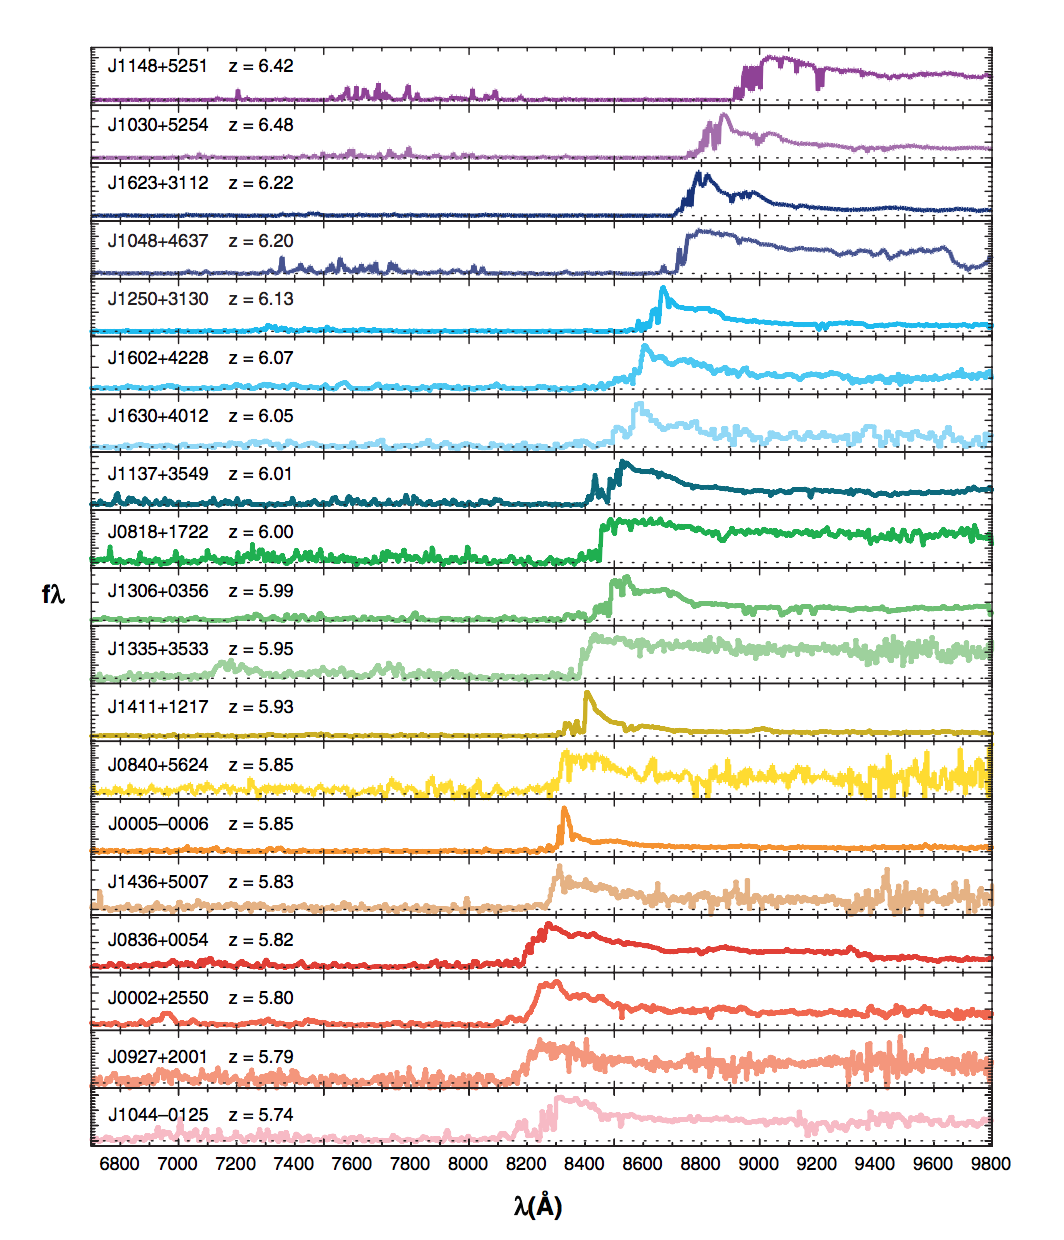
\includegraphics[width=0.8\textwidth]{chapters/eor_intro/figures/FanSpectra.png}
 \caption[The Ly$\alpha$ spectra of 19 high-redshift quasars.]{The Ly$\alpha$ spectra of 19 high-redshift quasars, as reported by \cite{Fan.06.2}. The effective optical depth towards each quasar increases with redshift, suggesting an evolution in the neutral fraction of the IGM. This figure was taken from \cite{Fan.06.review}.}
 \label{fig:eor_intro_qso}
 \end{figure}

Spectroscopic observations of high-redshift sources are relatively difficult to perform, and require large amounts of integration time. However, the distinctive Ly$\alpha$ limit in the spectra shown in Figure~\ref{fig:eor_intro_qso} is a distinctive property of high-redshift quasars. As an alternative, astronomers have developed a photometric method that is cheaper and easier to perform, called the ``Ly$\alpha$ dropout" technique. In this scheme, a survey will use an appropriate set of filters to probe a given redshift (imagine rectangles overlaid on the spectra in Figure~\ref{fig:eor_intro_qso}). If an excess is seen towards one galaxy in one filter, and very little signal is seen in the next-bluest filter, that galaxy may be considered a candidate high-$z$ quasar. With some modelling, the luminosity function of  Ly$\alpha$ dropout galaxies can be used to measure the mass distribution of galaxies as a function of redshift \citep[e.g.][]{Bouwens.15, Bouwens.16}. Using these luminosity functions and comparing to star formation rate models and measurements, \cite{Robertson.15} argue that current measurements are consistent with quasars playing a relatively minor role in reionization, with the bulk of ionizing photons arising form ``normal" galaxies rather than black hole accretion discs. However, this claim is moderately dependent upon uncertain model parameters, such as the escape fraction of ionizing photons from their local halo \citep{Robertson.13} and the star formation history at high redshifts. The latter is beginning to be answered as more high-redshift gamma-ray bursts are detected and characterized \citep{Wang.09, Robertson.12, Wang.15}.
%\footnote{In work unrelated to the bulk of this thesis, I presented observations of gamma-ray burst hosts suggesting that gamma-ray bursts were unbiased tracers of star formation rate -- a crucial component for using gamma-ray bursts to inform our understanding of the EoR \citep{Kohn.15}.}.

At the time of writing, photometric and spectroscopic observations of high-$z$ quasars suggest that the IGM had a neutral fraction $>10^{-4}$ at $z\sim 6$, indicating that the EoR ended around 1 Gyr after the Big Bang \citep{Barnett.17}. \cite{Fan.06.2} reported a direction dependence on their measurements, suggesting that reionization was patchy, rather than homogeneous.

\subsection{Observations of the CMB}
% CMB tau, kSZ
CMB photons will Thomson-scatter off-of free electrons in their path, suppressing the observed signal in a given direction. This suppression is described by an optical depth,

\begin{equation}
\tau_{\rm cmb} \propto \int^{z_{\rm recomb}}_0 x_i(z) a(z) \frac{{\rm d}l}{{\rm d}z}{\rm d}z,
\label{eq:eor_intro_tau_cmb}
\end{equation}
where $x_i(z)$ is the average ionized fraction at redshift $z$, $z_{\rm recomb}\approx1100$ is the redshift of recombination (and last scattering), $a(z) = (1+z)^{-1}$ and  ${\rm d}l/{\rm d}z$ is the cosmological line-element to redshift $z$. The optical depth to the CMB will suppress the observed primary anisotropies\footnote{The CMB is most-usefully described in harmonic $C_{\ell}$-space. Primary anisotropies, due to damped acoustic oscillations in the early hot plasma \citep{Silk.68}, are strongest at multipoles $\ell\lesssim3000$ -- equivalent to spatial scales $\theta \gtrsim 0.1^{\circ}$.} by a factor of $e^{-\tau_{\rm cmb}}$.

The dependence on $x_i(z)$ is crucial to our current understanding of the EoR; the largest contribution to the value of $\tau_{\rm cmb}$ will come from the large injection of electrons into the IGM during the EoR. Its measurement is not without complications: the suppression effect is degenerate with the overall amplitude of the CMB power spectrum, and it is an integrated quantity. 

The first complication can be addressed by performing polarized observations of the CMB, which breaks the degeneracy. A CMB photon that scatters off of an electron within a quadrupolar anisotropy will become linearly polarized, boosting polarized power at $\ell\sim2\sqrt{\tau_{\rm cmb}}$ \citep{Zaldarriaga.97.pol}. The WMAP satellite was the first telescope capable of making all-sky measurements of the CMB polarization, and detected an such an excess in polarized power, as shown in Figure~\ref{fig:eor_intro_spergel_tau} \citep{Kogut.03, Spergel.03}.

\begin{figure}
\centering
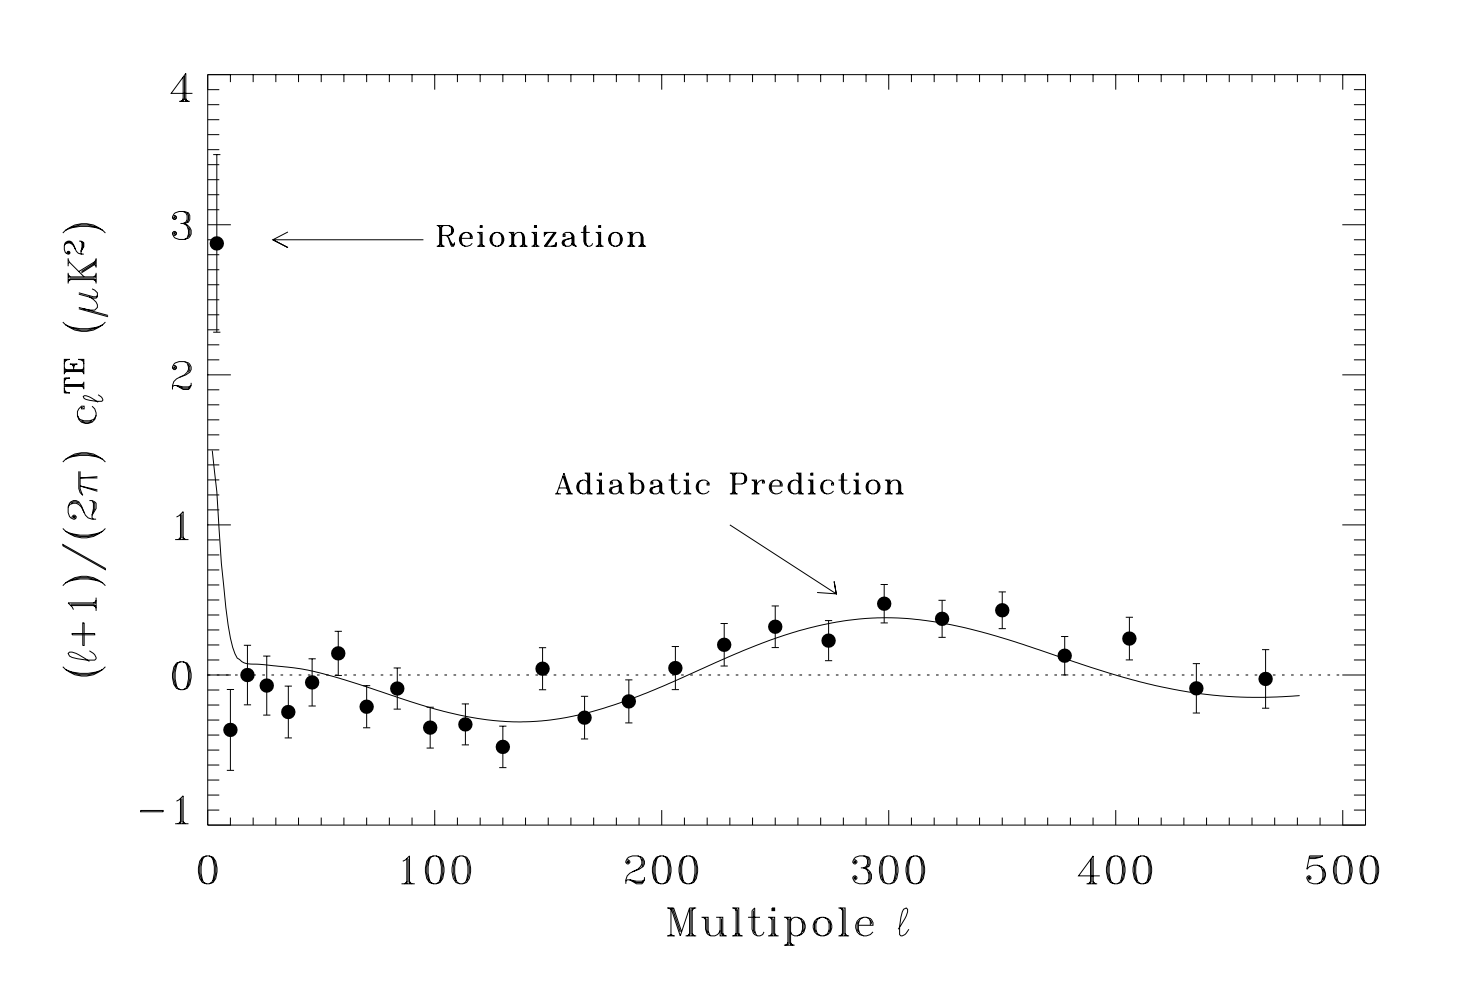
\includegraphics[width=0.8\textwidth]{chapters/eor_intro/figures/spergel_tau.png}
\caption[The $TE$ cross-power spectrum from WMAP.]{The Temperature-Linear Polarization ($TE$) cross-power spectrum from WMAP. The power was consistent with collisionless models save for an excess at large scales, consistent with large amounts of Thomson scattering of CMB photons during the EoR. Figure taken from \cite{Spergel.03}.}
\label{fig:eor_intro_spergel_tau}
\end{figure}

Such a measurement is able to recover a value of $tau_{\rm cmb}$, but due to its integral nature does not provide an ionization history. Values of $x_i(z)$ are therefore extremely model-dependent; typically extracted by assuming ``instantaneous reionization" in which $x_i(z)$ transitions from 0 to 1 quickly and smoothly. These models are often described using the tanh form:

\begin{equation}
x_i(z) \propto 1+\tanh\left(\frac{z - z_{\rm re}}{\Delta z}\right),
\end{equation}
where $z_{\rm re}$ is the redshift of instantaneous reionization, but is more usefully thought of as the redshift at which $x_i \approx x_{HI} \approx 0.5$. $\Delta z$ is the duration of reionization. Using such models, \cite{Planck.16.reionization} reported limits of  $7.8 < z_{\rm re} < 8.8$ and $\Delta z < 2.8$. They also reported that all of their modelling suggested that $x_i(z\gtrsim10)<0.1$.

The CMB provides us with more than one probe of reionization. \cite{Zeldovich.69} and \cite{Sunyaev.70} showed that CMB photons that scattered off of free electrons would introduce secondary anisotropies to the CMB (i.e. additional features in the $C_{\ell}$ spectrum). The Sunyaev-Zeldovich (SZ) effect is divided in to two categories: the thermal effect (tSZ) and the kinetic effect (kSZ). The tSZ occurs when CMB photons scatter off of electrons with high energies ($\sim 10$\,keV) due to their temperature; such high temperatures can only occur in high-mass galaxy clusters, and hence at redshifts lower than the EoR. 

The kSZ is of relevance to EoR studies. CMB photons scattering off of clouds of electrons in coherent velocity flows can be Doppler-shifted, which will redshift or blueshift (depending on the sign of the line-of-sight velocity) spectral observations of the CMB. Of course, clouds of electrons exist in relatively low-redshift galaxy clusters, and it was their contribution to the kSZ that was first detected \citep{Hand.12}. However, detection of the EoR contribution to the signal would be a powerful probe of dynamics on cosmological scales in the early Universe. The distortion induced by the kSZ on the CMB is given by

\begin{equation}
\frac{\delta T}{T_{\rm CMB}}(\hat{s}) = \frac{\sigma_T}{c} \int_0^{z_{\rm recomb}} n_e(z)e^{-\tau(z)} \hat{s}\cdot\vec{q} \frac{{\rm d}s}{{\rm d}z}{\rm d}z,
\end{equation}
where $\sigma_T$ is the Thomson Cross Section, $n_e(z)$ is the average number density of electrons at redshift $z$, $\tau(z)$ is the optical depth to redshift $z$, and d$s$/d$z$ is the cosmological line element to redshift $z$ along direction $\hat{s}$. We can model inhomogeneities in the ionization and baryon fraction as vector field
\begin{equation}
\vec{q}(\hat{s}) = (1+\delta_x)(1+\delta_b)\vec{v}(\hat{s}),
\end{equation}
where $1+\delta_x = x_i/\left\langle x_i \right\rangle$, $1+\delta_b= \rho_b/\left\langle \rho_b \right\rangle$ and $\vec{v}$ is the free electron bulk flow.

This is an optical depth effect much like the optical depth of the CMB in Equation~\ref{eq:eor_intro_tau_cmb}. However, it has important distinctive features: it is a direction dependent, probing the velocity of electron bulk flows along the line of sight, rather than the average ionization history, and it can create excesses and decrements in power, depending on the sign of the velocity component.

Detection of the kSZ is difficult, as the secondary anisotropies it causes in brightness temperature are a few percent of tSZ. Compared to the primary anisotropies, the tSZ is roughly 10 times weaker in $\mathcal{D}_{\ell}=(\ell+1)\ell C_{\ell}/2\pi^2$, and the kSZ is roughly 100 times weaker.
\cite{George.15} reported a detection of the kSZ at $\ell\approx3000$ (where the primary anisotropies and the Cosmic Infrared Background, a CMB contaminant at small scales, are both close to their minimum values), using a suite of cosmological and spectral models to remove CMB foregrounds, the primary anisotropies and the tSZ \citep[e.g.][]{Shaw.10}. Again, measurements from the CMB are integrated quantities, so their constraints on reionization are model dependent. Using a symmetric model of reionization history \citep{Zahn.12}, they set the constraint that $\Delta z < 5.4$, with their likelihood peaking around $\Delta z = 1.3$. Using similar techniques with shallower data from the same telescope, \cite{Zahn.12} set consistent limits that $\Delta z \geq 2$, and also that reionization ended at $z>5.8$.

Wide-field measurements of the kSZ would be rewarding, but the foregrounds of the Galaxy, CIB, CMB and tSZ represent contemporary challenges for direct-imaging experiments. However, one could hope to use correlations of the velocity field the kSZ sources, and the density field associated with it, to decorrelate the foregrounds and estimate the underlying fields \citep[e.g.][]{Cooray.04, Alvarez.16}. The mathematical formalism for such a technique is laid-out in Chapter~\ref{chapter:ksz_21cm}.

\section{Direct measurements of {\sc hi}}
\label{sec:eor_intro_hi}

To borrow a line from \cite{DannyThesis}, the Dark Ages were not dark. Our Universe is dynamic and energetic, and particles constantly seek a lower energy state.

Throughout the Dark Ages and the EoR, {\sc hi} was shining, weakly, at radio wavelengths. The {\sc hi} atom is capable of a hyperfine transition between its ${}_{1}s_{1}$ and ${}_{0}s_{1}$ energy levels. The electron spin can spontaneously change from parallel to the proton spin to antiparallel, emitting a photon of frequency $\nu_{21\,cm}\approx1420.4$\,MHz; a rest-wavelength of roughly 21\,cm. The emission coefficient of this transition is $\sim 2.9\times10^{-15}\,s^{-1}$, corresponding to a half-life of approximately 11 million years per atom. This is both the strength and the weakness of observing {\sc hi}. According to Fermi's Golden Rule, the probability of emission is equal to that of absorption; a small transition rate leads to a relatively dim signal, but 21\,cm photons are extremely unlikely to be observed between their emission and observation. This allows the 21\,cm signal to be tomographically mapped -- a sharp excess at the relevant frequency indicates a redshift -- and constructed into a 3D cube in space and time.

Observations of {\sc hi} during the Dark Ages and the EoR would directly constrain the ionization history of the Universe, allowing us to probe the evolution of the density field at high redshifts, the properties of the first stars, galaxies and black holes, and map the structure of the IGM as it evolves as a function of redshift. It would also represent the furthest baryons ever detected, and the largest volume of the Universe ever surveyed. This Section reviews the nature of the 21\,cm line during the EoR, and two parallel endeavours to detect it, using the monopolar signal (i.e. power averaged over the sky), and the anisotropic signal (power as a function of spatial scale).

\subsection{The 21cm transition}

As noted above, the probability of a single {\sc hi} atom undergoing the 21\,cm transition is exceedingly small. However, during the Dark Ages and the EoR, {\sc hi} was ubiquitous, and such transitions would be occurring constantly.
The relative occupancy of the hyperfine state in {\sc hi} is given by

\begin{equation}
\frac{N_1}{N_0} = \frac{g_1}{g_0} e^{-h\nu_{\rm 21cm}/k_B T_S},
\end{equation}
where $g_1$ and $g_0$ refer to the triplet and singlet states of the atom and are equal to 3 and 1, respectively. This Equation defines the spin temperature $T_S$, an analog of molecular excitation temperature for {\sc hi}. By solving the radiative transfer equation for this system in the Rayleigh-Jeans limit \citep[e.g.][]{MooreThesis}, we can write the brightness temperature of the emission as:

\begin{equation}
T(z) = T_S \tau_{\nu}(z) + T_{\rm bg}(1-\tau_nu(z)),
\label{eq:eor_intro_brightness_temp}
\end{equation}
where the optical depth of {\sc hi}, $\tau_{\nu}$, is assumed to be small, and the temperature of the background radiation $T_{\rm bg}$ is, for EoR observations, the temperature of the CMB at redshift $z$. \cite{Furlanetto.06} showed that the optical depth can be expressed in terms of cosmologically-interesting quantities, assuming the IGM is diffuse:

\begin{equation}
\tau_{\nu} \approx 9.2\times10^{-3} (1+\delta_b)(1+z)^{3/2}\frac{x_{HI}}{T_S}\frac{H(z)}{1+z}\frac{{\rm d}v_{\parallel}}{{\rm d}r_{\parallel}},
\end{equation}
where d$v_{\parallel}$/d$r_{\parallel}$ is the component of the peculiar velocity of the {\sc hi} cloud per unit depth along the line-of-sight, with respect to the Hubble expansion given by $H(z)/1+z$. The prefactor of $9.2\times10^{-3}$ justifies the assumption of small $\tau_{\nu}$ made above. Comparison to the optical depth for the Ly$\alpha$ line in Section~\ref{sec:eor_intro_current} emphasizes that {\sc hi} observations refer an opposite regime of EoR probes.

Combining the above equations, we can define the brightness contrast between redshifted {\sc hi} emission and the CMB,

\begin{equation}
\delta T \approx 9{\rm mK} \times x_{HI} (1+\delta_b)(1+z)^{1/2} \left( 1 - \frac{T_{\rm CMB}(z)}{T_S} \right)
\left( \frac{H(z)/(1+z)}{{\rm d}v_{\parallel}/{\rm d}r_{\parallel}} \right).
\label{eq:eor_intro_dT_reionization}
\end{equation}

Note that $\delta T$ can saturate if $T_S \gg T_{\rm CMB}$, and can become arbitrarily negative if $T_S \ll T_{\rm CMB}$. The observed emission is `backlit' by the CMB -- it's observability hinges on its relationship to $T_{\rm CMB}$.
Also note that the characteristic brightness temperature in Equation~\ref{eq:eor_intro_dT_reionization} is of order mK. By the time it is observed, the 21\,cm emission from the EoR has redshifted into meter wavelengths. At these wavelengths, Galactic synchrotron dominates the sky with brightness temperatures $\sim 10^3$\,K (see Chapter~\ref{chapter:astro_rad}; \citealt{McQuinn.07}). Foreground removal or avoidance remains the primary challenge for all EoR experiments, and will be discussed extensively throughout this thesis. I believe that the promises of 21\,cm tomography, outlined below, make the challenge worth pursuing. For a comprehensive reviews of the theory behind high-redshift 21\,cm tomography, see \cite{Madau.97}, \cite{Furlanetto.06} and \cite{Pritchard.10}. 

It is important to mention here, and will be re-iterated, that the 21\,cm photons generated through the hyperfine transition are highly unpolarized. Primordial magnetic fields could induce circular polarization via Zeeman splitting, but such an effect would be 3 to 4 orders of magnitude smaller than the already faint total intensity signal itself \citep[e.g.][also see Chapter~\ref{chapter:astro_rad}]{Babich.05}.

% spectral structure?

% why is it interesting (near term) - Liu Tau constraints, Kittiswitt maps (topology of EoR = cool), Kern emulators -- sensitivity to astrophysics & cosmology

\subsection{Global signal}
% WF coupling

The sky-averaged 21\,cm signal, sometimes called ``global signal", is a direct measurement of the spin temperature as a function of redshift. Equation~\ref{eq:eor_intro_brightness_temp} can be approximated as \citep{Field.56}:

\begin{equation}
T_S^{-1} = \frac{T_{\rm CMB}^{-1} + x_cT_K^{-1} + x_{\alpha}T_c^{-1} }{1 + x_c + x_{\alpha}}
\end{equation}
where $x_c$ and $x_{\alpha}$ are coupling coefficients for collisions and UV scattering, respectively, $T_K$ is the kinetic temperature of the gas, and $T_c$ is the effective temperature of the UV radiation field. The magnitude and sign of $T_S$ with respect to $T_{\rm CMB}$ is therefore proportional to each coupling constant.

At high redshifts, \cite{Wouthuysen.52} and \cite{Field.59} showed that there was good reason to expect that $T_c \rightarrow T_K$, such that $T_S$ decouples from $T_{\rm CMB}$. The effect -- now known as the Wouthuysen-Field Effect -- relies on Ly$\alpha$ radiation from early luminous sources exciting {\sc hi} in the ${}_1s$ states into the ${}_2p$ states. The atoms can then decay to the  ${}_1s_1$ state via allowed transitions, overpopulating that hyperfine energy level. This couples the {\sc hi} to the UV radiation field; the strength of the coupling depends on the spectral shape of the Ly$\alpha$ line. Increasing the coupling to UV scattering would make $T_S$ large and negative.

A fiducial reionization history is shown in Figure~\ref{fig:eor_global_signal_sketch} \citep{Mirocha.12}, with important turning points and zero-crossings highlighted. Working forwards through history, collisional coupling is relatively large in the Dark Ages, and couples $T_S$ to a low $T_K$, creating an absorption trough. The Universe continues to expand, baryon density drops, and $T_S$ and $T_K$ decouple; $T_S$ tends towards zero as it grows closer to $T_{\rm CMB}$.
As the first stars ignite, marking the end of the Dark Ages, their UV emission couples to the spin temperature via the Wouthuysen-Field Effect, creating a sharp absorption feature. As more massive structures form, X-rays begin to dominate the ionizing radiation field, increasing $T_K > T_{\rm CMB}$ such that the 21\,cm signal is seen in emission for the rest of the EoR. The 21\,cm spin temperature goes to zero, as it must, at the end of the EoR \citep[e.g.][]{Pritchard.10, Rao.17}. 

\begin{figure}
\centering
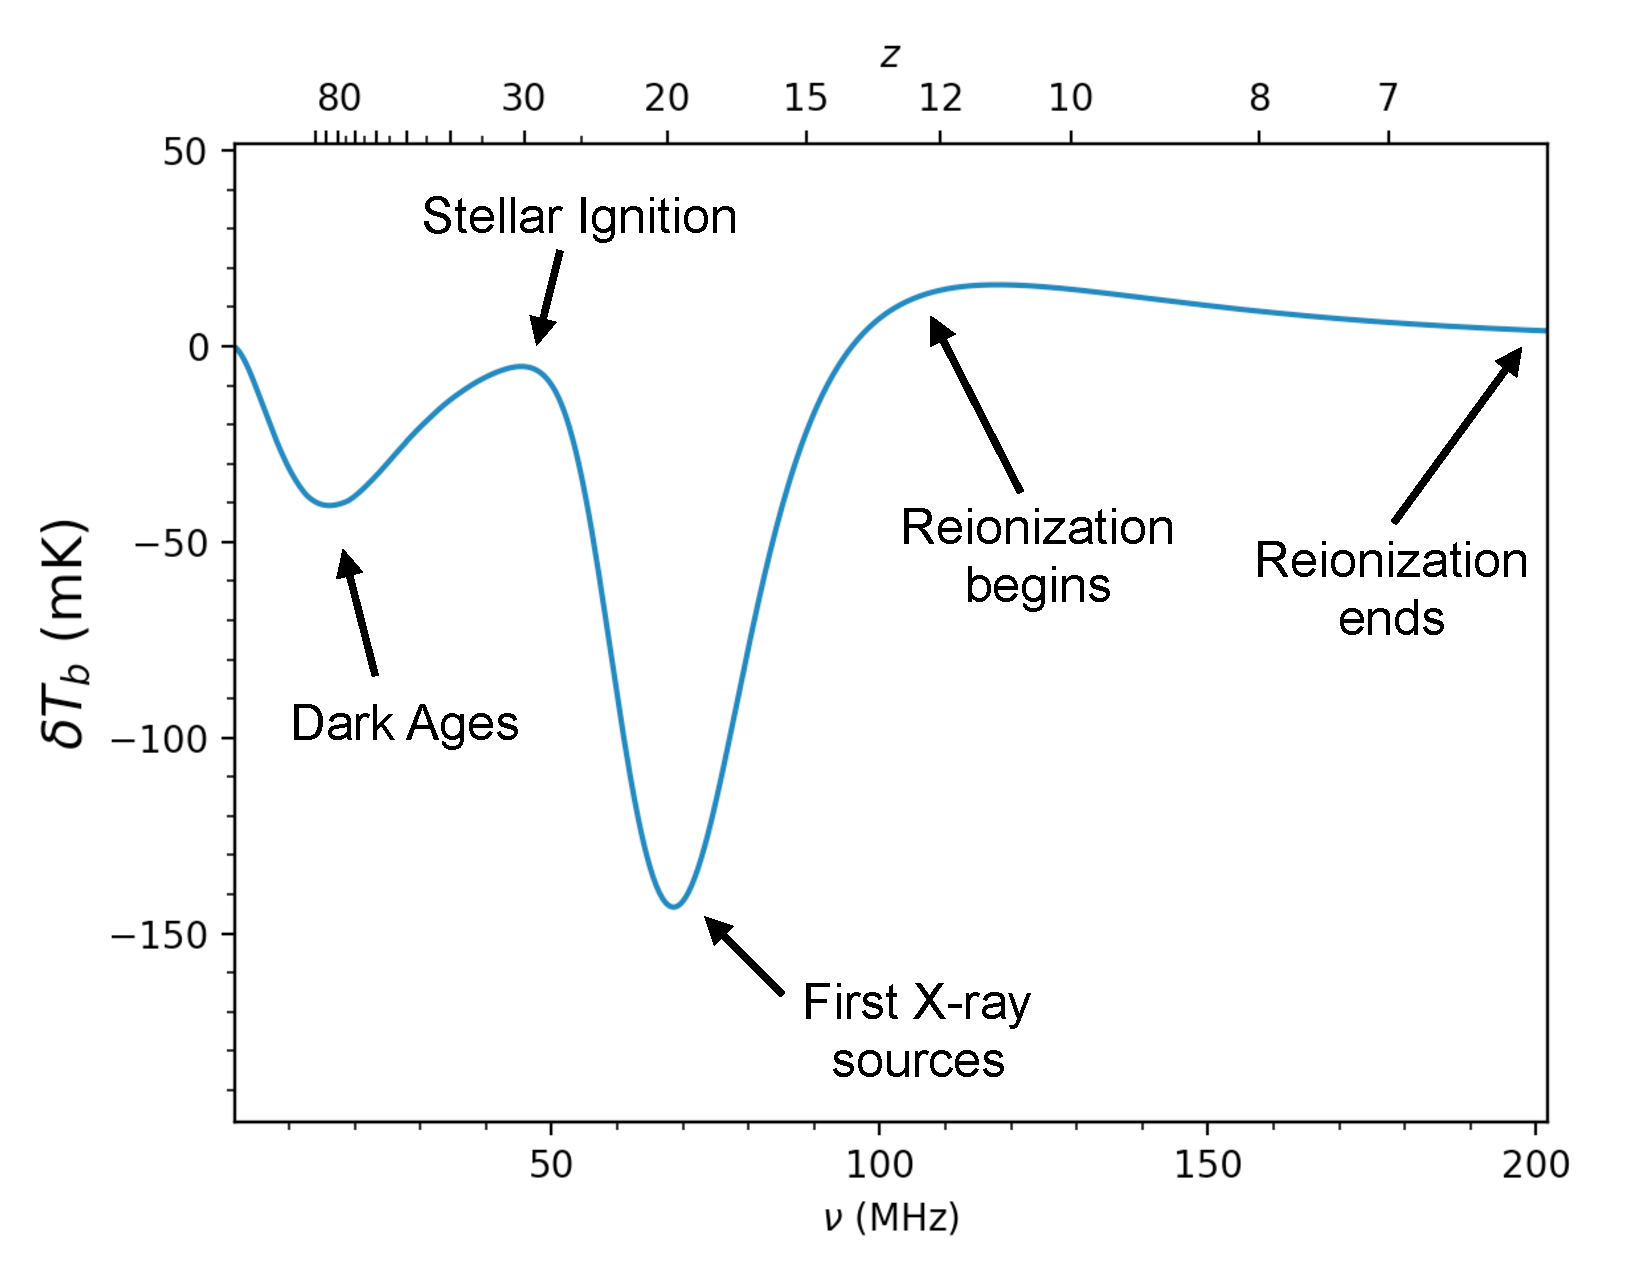
\includegraphics[width=0.8\textwidth]{chapters/eor_intro/figures/ares_sketch.pdf}
\caption[The history of the EoR global signal.]{The history of the EoR global signal, with important turning-points indicated. This figure was produced using the fiducial model of \cite{Mirocha.12}.}
\label{fig:eor_global_signal_sketch}
\end{figure}

Given the history described above, detection of the global signal would provide key information about the thermal history of the IGM as a function of redshift, and about the high-energy emission spectra of early stars and galaxies. Historically, observational efforts to detect the global signal have been ``single dish'' experiments, where a single receiving element is characterized to high precision, and then operated in an effort to detect the EoR signal as a function of frequency (and thus redshift). Such experiments typically seek to characterize the location and depth of the turning points, with the advent of X-ray sources giving the highest potential signal-to-noise. Experiments such as the Experiment to Detect the Global EoR Step (EDGES, \citealt{Bowman.10}), Sonda Cosmol\'{o}gica de las Islas para la Detecc\'{i}on de Hidr\'{o}geno Neutro (SCI-HI, \citealt{Voytek.14}), and the Cosmic Twilight Polarimeter (CPT, \citealt{Nhan.16}), have been proposed or constructed seeking to measure the global signal from the Dark Ages or the EoR, through a deep understanding of the properties of the instruments.

In all cases, the instruments consist of a single element, and much of the observational effort contributes toward a thorough understanding of systematic uncertainties of the instrument. Given that the signal is thought to be 4--5 orders of magnitude fainter than the foregrounds, an exquisite understanding of the correlated noise in these instruments is of the utmost importance. At the time of writing, the most mature global experiment is EDGES, an extremely well-characterized radio spectrometer. By subtracting a precise model of the foreground spectrum (\citealt{Rogers.08}, improved upon by \citealt{Mozden.17}), \cite{Bowman.10} were able to set a lower limit on the length of the reionization tail (and hence of the EoR itself) of  $\Delta z \geq 0.06$, ruling-out instantaneous reionization.

Excitingly, as this Chapter was being written, the EDGES team announced a detection of the X-ray heating turning point at 78\,MHz \citep{Bowman.18}. Their detected absorption trough was so deep, however, that it exceeds physical models for the (negative) magnitude of $T_S$. \cite{Bowman.18} and \cite{Barkana.18} suggested that the excess depth could be accounted for by additional collisions with dark matter. \cite{Ewall-Wice.18.edges} have shown that the excess could also be accounted for by an additional radio background from early black holes formed form Pop{\sc iii} stars. Confirmation from other global signal experiments will be required before the \cite{Bowman.18} result can be fully trusted, but it leaves open the possibility of {\sc hi} global signal experiments probing exotic particle physics, as well as astrophysics and cosmology.

\subsection{Anisotropic signal}

While the global signal may be computed by measuring the average brightness temperature at a given frequency, a richer astrophysical story can be told by measuring the anisotropies in the spin temperature at each redshift. Similarly to the CMB, these anisotropies can be represented through a 2-point correlation function; a power spectrum in Fourier space. Unlike the CMB, of course, this power spectrum  can be measured at each frequency observed, allowing us to construct a history of {\sc hi} emission on different spatial scales. 

Inspection of Equation~\ref{eq:eor_intro_dT_reionization} shows that the fluctuations will trace the underlying baryonic density field, but with a complicated bias depending upon the ionization fraction, peculiar velocities and importantly the nature of the ionizing sources, their clustering and their UV and X-ray spectra. This convolution of astrophysical and cosmological dependencies means that the redshift dependence of a given Fourier mode will give clues about the ionization history. Maxima represent high contrasts in the brightness temperature field, suggesting middle stages of the EoR. However, the bulk of information contained in power spectra will require models to extract. This requirement is not as onerous as it might sound, thanks to decades of theoretical work (an exhaustive list is impossible, but the literature reviews of \citealt{Grieg.17} and \citealt{Kern.17} provide useful starting points). 

For example, Figure~\ref{fig:eor_intro_liu_history} shows the enormous improvement in modelling the ionization history, given high signal-to-noise measurements of the 21\,cm power spectrum. Including {\sc hi} data leads to precise constraints on $x_{HI}(z)$ -- but the constrains may be inaccurate in their timing of the EoR without including CMB polarization measurements. 

\begin{figure}
\centering
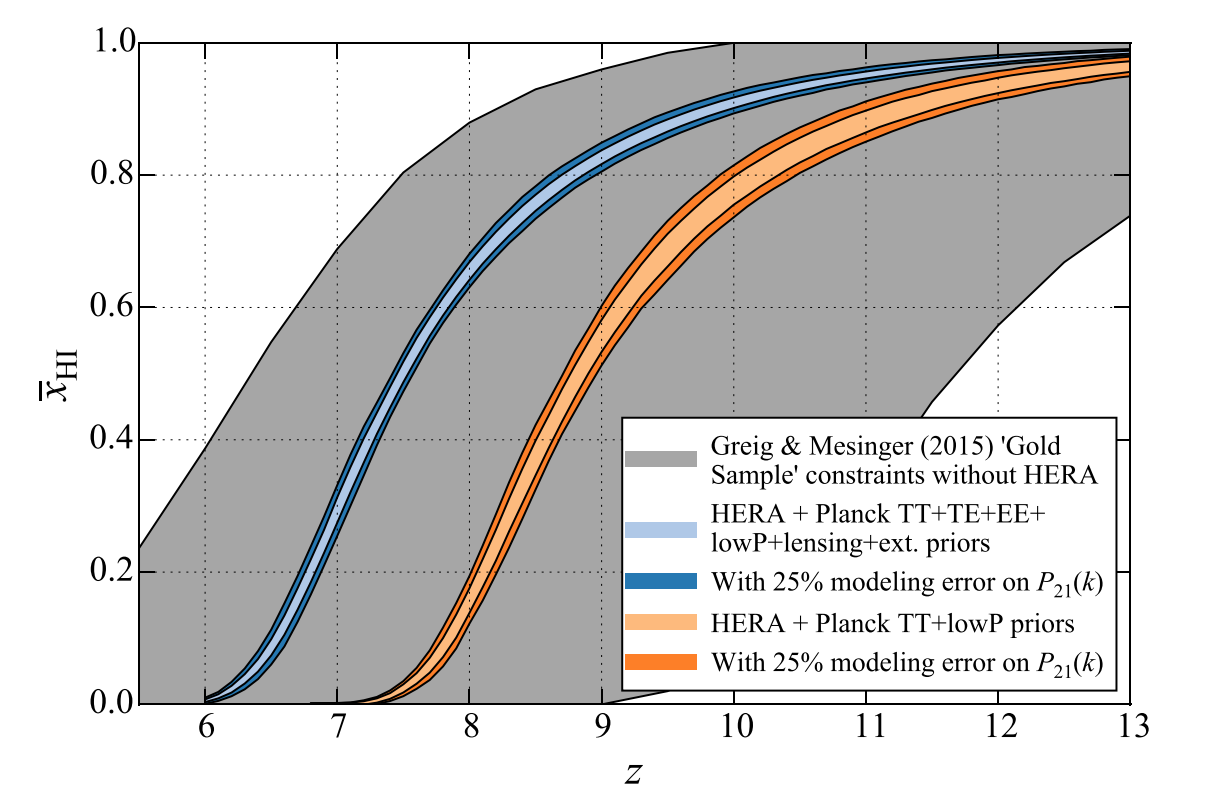
\includegraphics[width=0.7\textwidth]{chapters/eor_intro/figures/Liu_history.png}
\caption[Forecasts for constraints on the ionization history, given high signal-to-noise measurements of the {\sc hi} power spectrum at each redshift from HERA.]{Forecasts for constraints on the ionization history, given high signal-to-noise measurements of the {\sc hi} power spectrum at each redshift from HERA. The grey band shows constraints on the ionization history without measurements of {\sc hi}, while the blue and orange curves include power spectrum measurements in their modelling. Without CMB polarization measurements, an shift in the timing of reionization can occur. Figure taken from \cite{Liu.16}.}
\label{fig:eor_intro_liu_history}
\end{figure}

As discussed in Section~\ref{sec:eor_intro_current}, parametrizing the optical depth to the CMB can grant a model-dependent measurement of the ionization history, but one must rely on models in which reionization occurs very quickly. Curves such as those shown in Figure~\ref{fig:eor_intro_liu_history} would eliminate the need for such models by providing a measurement of the ionization history. This in turn can break degeneracies in other measurements from the CMB. For example, \cite{Liu.16.tau} showed that estimates of the sum of neutrino masses\footnote{Understanding the sum of the masses of the three flavors of neutrinos is a critical measurement in the realm of quantum chromodynamics. It is informed by the CMB, as neutrinos can suppress the formation small-scale anisotropies.} can be improved by $\sim10\%$ -- importantly, with likelihood contours perpendicular to other probes.

\cite{Kern.17} used machine-learning techniques to generate a suite of emulators for the {\sc hi} power spectrum. Given measurements of the power spectrum as a function of redshift, with realistic errors and foreground mitigation, their emulators would be able to constrain cosmological and astrophysical parameters for the EoR and the Dark Ages to relatively high precision. Their constraints on astrophysical parameters were tighter than cosmological ones due to the fact that the brightness contrast is a complicated proxy for the cosmic density field. To illustrate this complication, we show slices of simulation cubes in Figure~\ref{fig:eor_intro_plp_sim}, showing the baryon density field and the corresponding 21\,cm brightness temperature close the middle of the EoR. In the bottom panel, we show the evolution of the 21\,cm field along the line of sight, emphasizing that EoR measurements can provide a rich history of the IGM.

\begin{figure}
\centering
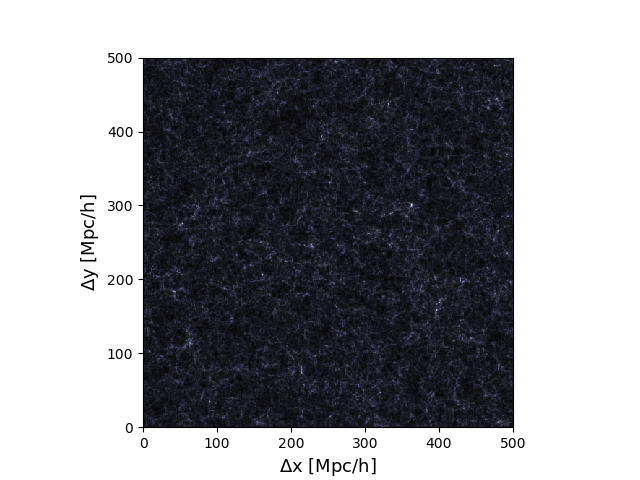
\includegraphics[width=0.5\textwidth]{chapters/eor_intro/figures/density.png}
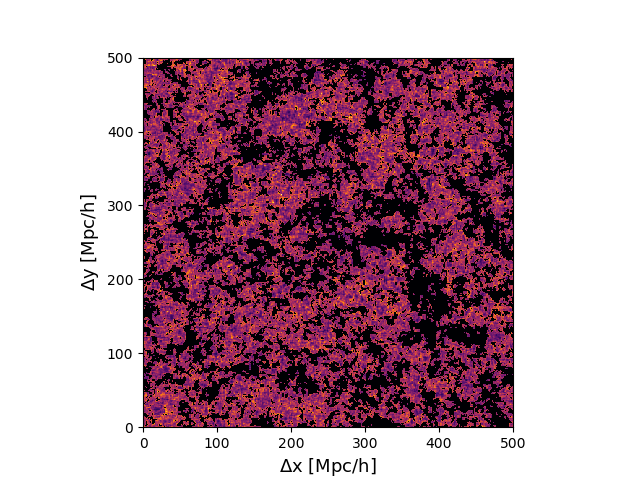
\includegraphics[width=0.5\textwidth]{chapters/eor_intro/figures/t21.png}
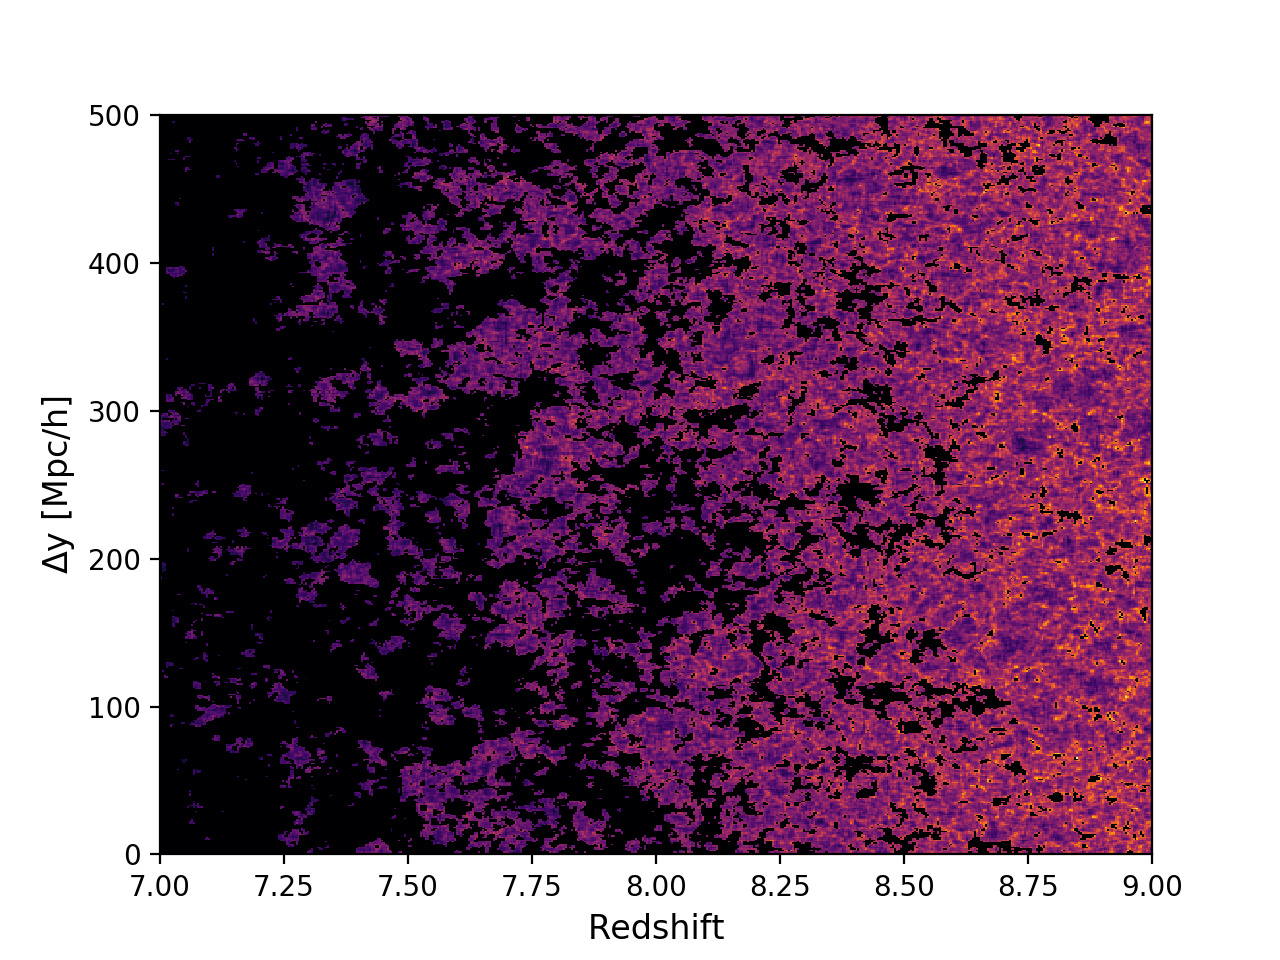
\includegraphics[width=0.5\textwidth]{chapters/eor_intro/figures/t21_z.png}
\caption[An example cosmological simulation of the EoR and the corresponding density field.]{An example cosmological simulation of the EoR. The upper panel is the baryon density field, and middle one is the corresponding 21\,cm brightness contrast, both at redshift $z\sim 8$. Both fields have been normalized for this illustration, the purpose of which is to show that there is not a simple mapping between the cosmological density field and the {\sc hi} observable. The bottom panel shows the 21\,cm brightness contrast as a function of redshift.}
\label{fig:eor_intro_plp_sim}
\end{figure}

Moving beyond statistical measurements to maps of the EoR\footnote{The reason for this order is due to the strength of the foregrounds, and strategies employed mitigate them. These will be explored at length in Chapter~\ref{chapter:eor_window_theory}.} opens a rich window for observational cosmology. Performing real-space tomography would allow us to construct cubes of the {\sc hi} field at different redshifts. Studying the shape and size of bubbles would provide us with a way to identify individual ionizing sources and interpret them. \cite{Robertson.15} showed that there are barely enough galaxies to account for the ionization of the Universe, suggesting that other sources such as quasars must play a role -- the signature of which would be detectable in tomographic cubes (Chapter~\ref{chapter:hera_ml}, shows an initial machine learning framework to perform this characterization). % more imaging things?

Radio interferometers (see Chapter~\ref{chapter:interferometry}), are excellent instruments for probing temperature anisotropies, and their measurements naturally translate into the Fourier space native to power spectrum measurements (see Chapters~\ref{chapter:instruments} and \ref{chapter:eor_window_theory}). Interferometers currently pursing detection of the EoR power spectrum include the Giant Meterwave Radio Telescope \citep[GMRT;][]{Paciga.13}, the Low Frequency Array \citep[LOFAR;][]{vanHaarlem.13}, the Murchinson Widefield Array \citep[MWA;][]{Tingay.13}, the Donald C. Backer Precision Array for Probing the Epoch of Reionization \citep[PAPER;][]{Parsons.10} and the Hydrogen Epoch of Reionization Array \citep{deBoer.17}.

Low-frequency radio interferometers such as those listed above have not yet reported results of sufficient depth to claim a detection of the EoR power spectrum. This is largely due to the major challenge faced by all EoR experiments -- extremely bright foregrounds. The intensity of the synchrotron radiation that dominates the low-frequency sky scales as a power law in frequency, so probing higher and higher redshifts becomes more and more difficult (see Chapter~\ref{chapter:astro_rad}). As we discuss in Chapter~\ref{chapter:eor_window_theory}, the chromatic response of an interferometer may provide a crucial lever arm for disentangling foreground and background radiation. The instrument itself also behaves as a foreground, as at such low frequencies, thermal noise in the electronics is a much larger fraction of the `observed' signal than redshifted 21\,cm emission.

\section{Current Limits and Future probes}
\label{sec:eor_intro_future}

Over the past decade, immense progress has been made to constrain the global history of the EoR. To review a few limits that have been discussed in this Chapter, limits from quasars and the kSZ have set the end of reionization $5.8 < z_{\rm end} < 6.0$. Measurements of the optical depth to the CMB have set model-dependent limits that put the middle of reionization at $7.8 < z_{\rm mid} < 8.8$. Combining kSZ measurements with the optical depth of the CMB has set an upper limit on the duration of the EoR, and measurements from EDGES have set a lower limit, such that $0.06 < \Delta z < 2.8$.

Current kSZ limits and low-significance detections, and measurements from quasars, are consistent with a patchy EoR -- bubbles opening to create an inhomogeneous spin temperature field. Figure~\ref{fig:eor_intro_pspec_limits} shows current limits on the EoR power spectrum from radio interferometers, as a function of redshift {\color{red} (Kolopanis et al., in prep.)}. The limits correspond to different spatial scales, but until some scale-dependence of the EoR power spectrum is detected, plotting them along side one another is valid. Integrations are becoming successively deeper, but there is a ways to go, as shown by a fiducial reionization power spectrum curve \citep{Mesinger.11}. Deeper integrations require more interferometric baselines and longer observing seasons, both of which require precision calibration and control of instrument systematics. New techniques for some of these challenges are presented in Part {\sc ii}.

\begin{figure}
\centering
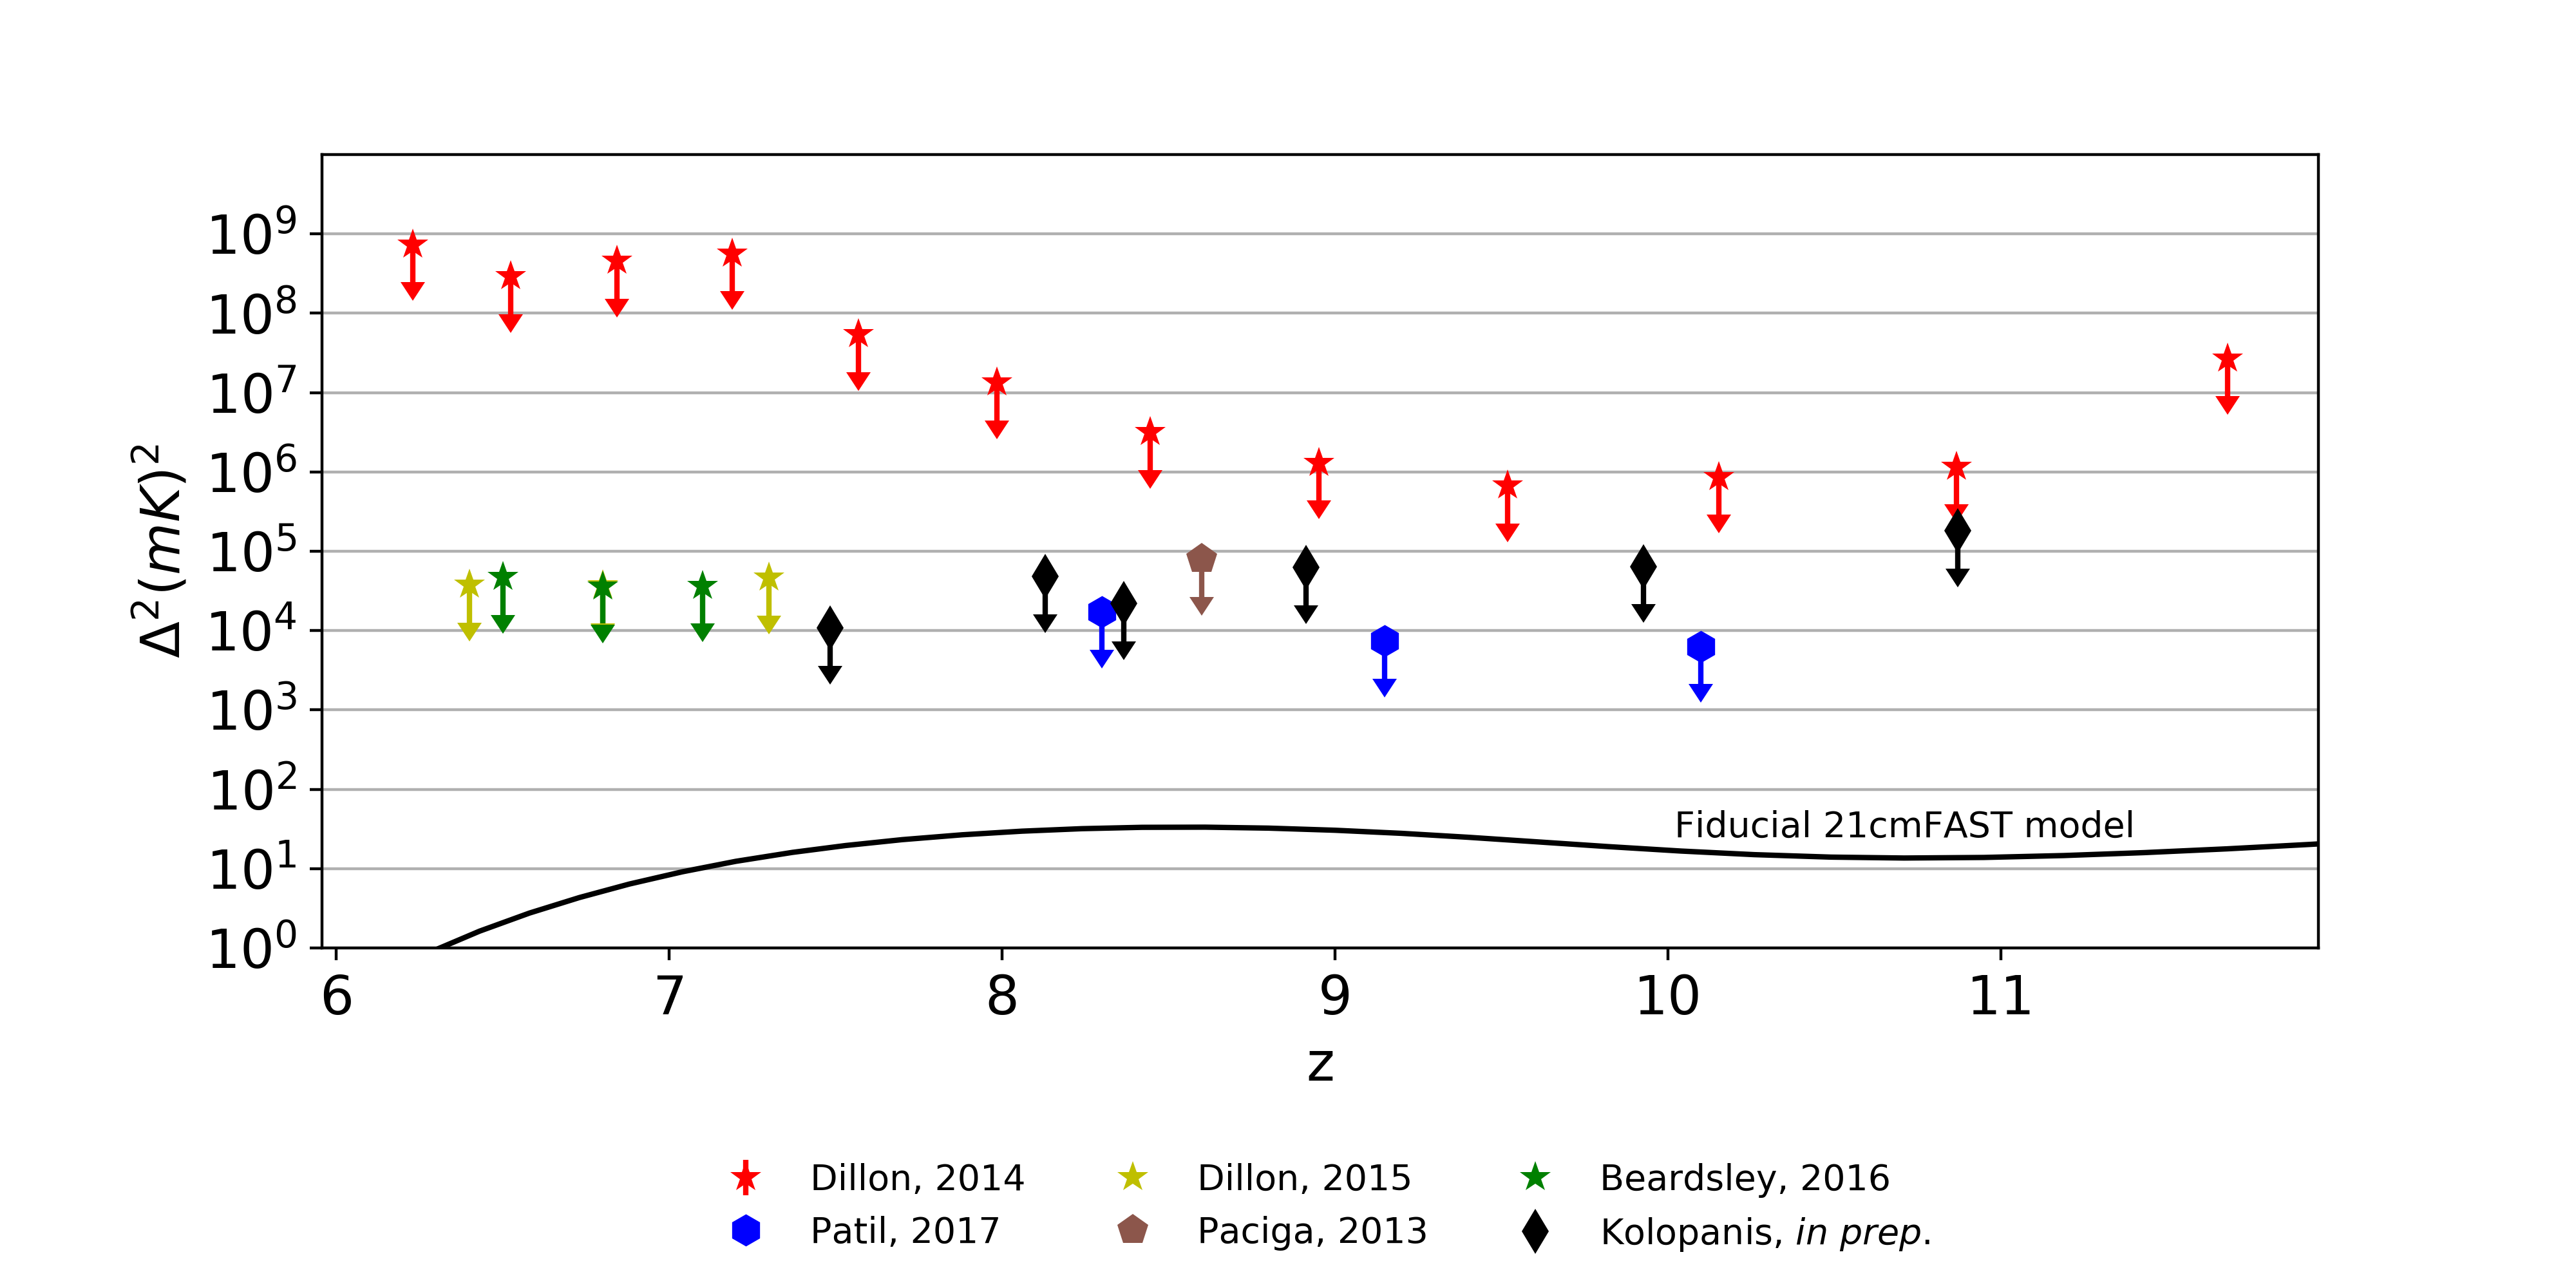
\includegraphics[width=0.8\textwidth]{chapters/eor_intro/figures/eor_lowest_limits.png}
\caption[Current limits on the EoR power spectrum, as a function of redshift.]{Current limits on the EoR power spectrum, as a function of redshift. Different symbol shapes correspond to different instruments, with stars \citep{Dillon.14, Dillon.15, Beardsley.16} indicating measurements from the MWA, blue hexagons \citep{Patil.17} from LOFAR, the brown pentagon from the GMRT \citep{Paciga.13} and the black diamonds from PAPER-64 {\color{red} (Kolopanis et al., in prep.)}. Figure taken from {\color{red} Kolopanis et al., in prep}. Plotted beneath all of the limits is a fiducial 21\,cm power spectrum \citep{Mesinger.11} -- there is still a factor of $\sim 10^3$ to integrate-down upon.}
\label{fig:eor_intro_pspec_limits}
\end{figure}

This Chapter has reviewed our current understanding of the EoR, and why it's observation would represent an enormous advancement for modern cosmology. The pursuit of realizing 21\,cm tomography is relatively mature, but other atomic transitions could contain similar promise. \cite{Silva.13} suggested that one could perform an intensity-mapping survey of Ly$\alpha$ emission. Such an experiment would involve several narrow-band filters to extract the high-redshift Ly$\alpha$ power spectrum at $z\sim7$, statistically probing the population of ionizing sources towards the end of the EoR, when Ly$\alpha$ is detectable. Narrow-band surveys for Ly$\alpha$ emission yielded a possible detection of Pop{\sc iii}-like stars at $z\sim 6.6$ \citep{Sobral.15}.

Carbon is easily ionized by diffuse starlight. The forbidden [C{\sc ii}] transition in ionized carbon could be used to perform tomography with advantages similar to {\sc hi}, as a probe of star formation history. At EoR redshifts, the emission line would redshift into an atmospheric window detectable in the Far Infra-red from Earth \citep[e.g.][]{Gong.12, Hunacek.16, Pentericci.16}. 
The polar nature of the CO molecule leads to a quantization of its energy states in integer multiples if its angular momentum, appearing as a `ladder' of emission lines that can be used for extremely precise redshift determination, and the relative intensity of which are determined by the temperature of the molecular cloud. Intensity mapping CO emission could provide a cosmic history of star forming giant molecular clouds \citep[e.g.][]{Righi.08,Lidz.11.CO}.
It is worth mentioning that all of these intensity mapping proposals suggest cross-correlation with 21\,cm tomographic measurements as a central science objective.

The James Webb Space Telescope is scheduled to launch between October 2018 and June 2019, and will be the most sensitive infra-red telescope ever constructed \citep{jwst}. It is predicted to be able to detect small mass halos ($\sim 10^5 M_{\odot}$) at $z\sim 10$ in its planned ultra-deep integrations \citep{Salvaterra.11, Zackrisson.11}. Its relatively small field of view will not allow for comprehensive surveys of the high-redshift Universe or the EoR, but correlating its measurements with 21\,cm maps would provide a probe of the dependence of high-redshift galaxies on their ionization environment \citep[e.g.][]{Beardsley.15}.

\section{This thesis}
\label{sec:eor_intro_this_thesis}
Everything in this work -- algorithmic development, mathematical theory, observations -- was carried-out in order to facilitate the detection of the EoR. While these efforts took many forms, they shared that singular motivation of moving the field forward, towards a detection of {\sc hi} anisotropies at cosmological distances. 

This thesis is divided into three parts. Part {\sc i} is devoted to introducing concepts used throughout this work and building a mathematical formalism around those concepts. 
Chapter~\ref{chapter:astro_rad} reviews astrophysical mechanisms for producing polarized and unpolarized radiation at low radio frequencies. 
Chapter~\ref{chapter:interferometry} builds a formalism around measuring low frequency radio waves with interferometers (and the challenges associated with accurately measuring polarized radiation), and Chapter~\ref{chapter:instruments} introduces the instruments used throughout this work.

In Part {\sc ii} I present the bulk of my efforts: building an understanding of the imprint of the polarized sky, and the instrument itself, in the Fourier space used to set limits on the EoR power spectrum. 
Chapter~\ref{chapter:eor_window_theory} reviews the current theory and major results of mapping low frequency interferometric measurements into Fourier space. 
Chapter~\ref{chapter:data_prep_and_proc} details several required quality assurance and compression steps that must be taken to clean and interact with the data. Building from clean data, Chapter~\ref{chapter:polcal} presents new algorithms developed to calibrate the measurements.
Chapter~\ref{chapter:ionosphere} discusses the impact of Earth's ionosphere on our measurements.
In Chapters~\ref{chapter:eor_window_paper32img}, \ref{chapter:eor_window_HERA} and \ref{chapter:eor_window_psa128} I present successively-deeper integrations on polarized foregrounds in successively-narrower regions of Fourier space.

Part {\sc iii} explores other uses of EoR measurements, beyond detection of the power spectrum. In Chapter~\ref{chapter:TAV}, I discuss the potential of using long time-averages of interferometric measurements to measure some component of the monopole moment of the sky. In Chapter~\ref{chapter:ksz_21cm}, I present a new formalism for cross-correlating 21\,cm emission and CMB anisotropies in Fourier space. Chapter~\ref{chapter:hera_ml} describes my initial investigations into utilizing deep learning techniques for recovering cosmological parameters from simulated EoR measurements. I conclude in Chapter~\ref{chapter:conc}.
